%%%%%%%%%%%%%%%%%%%%%%%%%%%%%%%%%%%%%%%%%%%%%%%%%%%%%%%%%%%%%%%%%%%%%%%%%%%%%%%%
%%% Methods
%%%%%%%%%%%%%%%%%%%%%%%%%%%%%%%%%%%%%%%%%%%%%%%%%%%%%%%%%%%%%%%%%%%%%%%%%%%%%%%%

\clearpage
\section{Methods and implementation}

In this section I will go over the methods I implemented to solve the given problem.
I will also introduce the technology choices and explain how they were used to implement the methods. \nyi{nyi}

\subsection{Chosen technologies}

The decision about which technologies I would use for my project was straightforward.
Since the project was to integrate with the existing Jury system, I chose to use shared technologies and libraries.
Jury was built with C\#, running as an ASP.NET MVC application with the .NET runtime \nyi{cite? version?}.
The database was running on SQL Server, and the query engine was set up with a object-relational mapping tool called Entity Framework. The approach used was a ''data first'' model, where the system automatically generates models (classes in code) based on the database schema. \nyi{links, citations}
The user provided text queries were translated to database queries with LINQ. \nyi{elaborate?}
I used these same technologies in my project.

\subsection{Graph construction}
\subsubsection{Pre-processing}

To comply with the user requirements of being able to generate models from custom queries and real-time production data, the system developed in this thesis should be able to take any set of events as the input.
As outlined before, the system should use the textual query system to retrieve the events from the database.
The system will not have any knowledge of what filtering has been used, it only executes the user-given query.
The only check the system needs to do is to check the events against the current user's permissions, to protect confidential information.

The Jury system already had functionality to retrieve the events from the database based on a \emph{query}.
A query is a string containing user-provided criteria for which events to show.
This could for example be querying for a specific product or a specific submission ID.
The result of the query was a plain timestamp-ordered list of events, as seen in figure \ref{fig:plaineventlog}.
After the query has been executed, the result is a set of events.
Because of the challenges outlined in section \ref{sec:datachallenges}, a pre-processing step is needed.

The pre-processing method chosen takes a set of events as the input. The pre-processing works as follows:
\begin{enumerate}
    \item Drop events based on the user's permission level.
    \item Group all events by \textbf{submission ID}.
    \item Create a trace corresponding to a submission for each group.
    \item Order all events in each trace by ascending timestamp, then by event ID.
    \item Drop all traces with an erroneous event such as ''Failed''.
    \item Drop all non-final events from each trace.
\end{enumerate}
After these steps the result is a set of valid traces, each corresponding to a unique submission ID with only final events.

By using different time slices or different filters on which events to include, we can generate models for different purposes. 
For example, we can try to generate a more accurate process model by filtering.
If we filter the events in the pre-processing step to only include events related to certain products
or product types, we can assume that the process model and the statistics will better describe those products.
However, filtering reduces the number of events used for the model, which can lead to overfitting.
\nyi{some theory here? overfitting? explain?}

\begin{figure}[htb]
    \centering 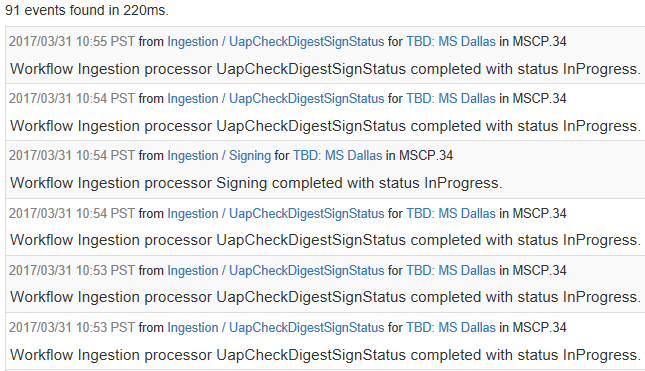
\includegraphics[width=0.7\linewidth]{gfx/plaineventlog.png}
    \caption{Event log query result view in Jury}
    \label{fig:plaineventlog}
\end{figure}

In my implementation I use the existing queries in Jury to retrieve events from the database. The queries can be written by users and saved in the system.
These saved queries are then used to discover the process models.
Each model corresponds to the query.
For example, if the query searches for events belonging to only game products, then the discovered process model will reflect the underlying process for games.
This allows for a highly flexible system where the users can create models for any subset of products or events they desire. 

\subsubsection{Creating directed graphs}

The model chosen to represent the process models is the directed graph. 
In this model, every pair of directly subsequent events $(a,b)$ appearing in a trace corresponds to a 
graph edge from node $a$ to node $b$.
The parallelism is generated by observing the direct follow-relations as in the \textalpha-algorithm.

To generate a graph from a set of traces, I started by generating an event log \emph{footprint matrix}.
The footprint matrix describes the relation of all the events in the event log regarding to each other.
This means that the matrix describes which events immediately follow another events in the set of traces.
The columns and rows of the matrix correspond to all the distinct activities (the vocabulary).
The matrix is square and should have a zero diagonal.
The row describes the first event, and the column the event directly following.
The number in the cell describes the frequency that this follow relation was observed in the logs (follow-frequency matrix).
This matrix can be generated by linearly traversing each trace once, and for each pair of events incrementing the number in the corresponding cell.

I will illustrate this with an example. Consider an event log with four activities $a,b,c,d,$ and $e$.
Figure \ref{fig:exampletraces} illustrates the six traces in the event log. There are two unique kinds of traces, $abcde$ and $acbde$, both of which have been observed three times. Figure \ref{fig:examplematrix} shows the footprint matrix generated from these traces.
The diagonal is zeroes, since no event follows itself.
From the upper triangle the matrix shows for example that $b$ has followed $a$ three times and $c$ has followed $b$ three times. From the lower triangle we see for example that $a$ has never followed $b$, but $b$ has followed $c$ three times.
By comparing the frequencies in the upper triangle to the lower triangle we can discover dependencies suggested by the event log, and from a lack of dependency we can suggest parallelism.

\begin{figure}
    \centering
    % example traces
    \begin{subfigure}[h]{0.4\linewidth}
        \begin{center}
        \begin{tabular}{| r | l |}
        Trace & Frequency \\
        \hline
        a b c d e & 3\\
        a c b d e & 3 \\
        \hline
        \end{tabular}
        \end{center}
        \caption{A list of example traces}
        \label{fig:exampletraces}
    \end{subfigure}
    % footprint example
    \begin{subfigure}[h]{0.4\linewidth}
        \begin{center}
        \begin{blockarray}{cccccc}
          & a & b & c & d & e\\
        \begin{block}{c(ccccc)}
        a & 0 & 3 & 3 & 0 & 0 \\
        b & 0 & 0 & 3 & 3 & 0 \\
        c & 0 & 3 & 0 & 3 & 0 \\
        d & 0 & 0 & 0 & 0 & 6 \\
        e & 0 & 0 & 0 & 0 & 0 \\
        \end{block}
        \end{blockarray}
        \end{center}
        \caption{An example footprint (follow-frequency) matrix $M$ }
        \label{fig:examplematrix}
    \end{subfigure}
    \caption{Example for traces containing events $\{a,b,c,d,e\}$}
\end{figure}

% turning the matrix into a graph
The generated footprint matrix corresponds directly to the log-based ordering relations described by van der Aalst and van Dongen \cite{van2013discovering,van2016process}.
There are four possible relations between any two events in an event log $L$:
\begin{itemize}
    \item $a \rightarrow_L b$: $b$ \emph{directly follows} $a$.
    \item $a \leftarrow_L b$: $b$ \emph{directly precedes} $a$.
    \item $a ||_L b$: $a$ and $b$ are \emph{parallel}.
    \item $a \#_L b$: $a$ and $b$ are not directly related, they are $unrelated$.
\end{itemize}

Note that it always applies that $a \rightarrow_L b \Leftrightarrow b \leftarrow_L a$.
We can find these relations from the footprint matrix by comparing each cell $m_{ij}$ the upper triangle with the corresponding cell $m_{ji}$ lower triangle by using the following algorithm:

\begin{definition}
Let $A = \{ a_i | 0 < i \le n \}$ be a set of $n$ activities (the \emph{vocabulary}).
Let $M$ be an $n \times n$ footprint matrix corresponding to $A$.
For each cell $m_{ij} \in M$ where $i < j$:
\begin{itemize}
    \item $a \#_L b$ iff $m_{ij} = 0$ and $m_{ji} = 0$
    \item $a_i \rightarrow_L a_j$ iff $m_{ij} > m_{ji}$ and $m_{ji} = 0$
    \item $a_i \leftarrow_L a_j$ iff $m_{ij} < m_{ji}$ and $m_{ij} = 0$
    \item $a_i ||_L a_j$ iff $m_{ij} > 0$ and $m_{ji} > 0$
\end{itemize}
Furthermore, it should be noted that these relations are symmetrical:
\begin{itemize}
    \item $a \#_L b \Leftrightarrow b \#_L a$ 
    \item $a_i \rightarrow_L a_j \Leftrightarrow a_j \leftarrow_L a_i$
    \item $a_i ||_L a_j \Leftrightarrow a_j ||_L a_i$ 
\end{itemize}
\label{def:logrelations}
\end{definition}

In the example, comparing the cell $M[a,b] = 3$ to cell $M[b,a] = 0$ we get $a \rightarrow b$. \nyi{formatting?}
However, by comparing $M[b,c] = 3$ to $M[c,b] = 3$ we see that $b || c$. 
Figure \ref{tab:examplefootprint} shows the generated footprint for the matrix shown in figure \ref{fig:examplematrix}.
Note that it is enough to only examine the upper triangle of the matrix, since the generated footprint is always symmetrical across the diagonal.
If the rows and columns are ordered by dependency, the dependencies follow the diagonal of the footprint.
The parallel activities can be seen visually as square-shaped symmetric regions.
The parallel region border consists of follow-relations while the inside of the region contains parallel-relations.
This shape can be seen in the example figure \ref{tab:examplefootprint}.

This footprint maps directly to a corresponding directed graph.
Every activity in the vocabulary corresponds to a graph node.
Every ''directly follows'' relation corresponds to a directed edge in the graph. A parallel relation corresponds to arcs in both directions.
Figure \ref{fig:examplegraph} shows the directed graph corresponding to the footprint from figure \ref{tab:examplefootprint}.

\begin{figure}
    \centering
    % footprint table example
    \begin{subfigure}[h]{0.4\linewidth}
        \begin{center}
        \begin{tabular}{cccccc}
        \hline
          & a & b & c & d & e\\
        \hline
        a & \# & $\rightarrow$ & $\rightarrow$ & \# & \# \\
        b & $\leftarrow$ & \# & || & $\rightarrow$ & \# \\
        c & $\leftarrow$ & || & \# & $\rightarrow$ & \# \\
        d & \# & $\leftarrow$ & $\leftarrow$ & \# & $\rightarrow$ \\
        e & \# & \# & \# & $\leftarrow$ & \# \\
        \hline
        \end{tabular}
        \end{center}
        \caption{Generated footprint of log relations}
        \label{tab:examplefootprint}
    \end{subfigure}
    % directed graph example
    \begin{subfigure}[h]{0.4\linewidth}
        \centering 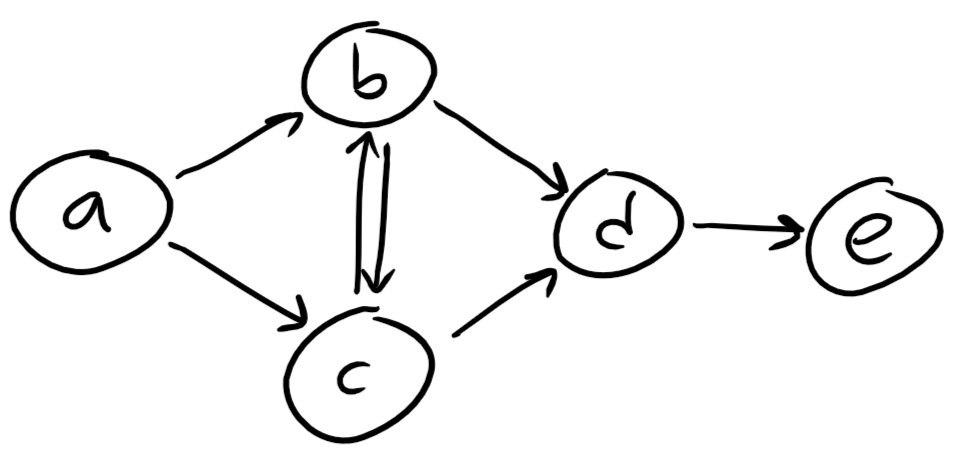
\includegraphics[width=\linewidth]{gfx/graphthing.jpg}
        \caption{Generated graph \nyi{remake}}
        \label{fig:examplegraph}
    \end{subfigure}
    \caption{Graph generation from the footprint}
\end{figure}

% Dealing with noise
Noise in the event log data creates problems if it is not appropriately handled. 
Network delays, bugs, and outages cause events to get lost or erroneously arranged. 
This noise manifests in the footprint follow-frequency matrix.

Figure \ref{fig:examplenoise} shows an example footprint matrix from a slice of production logs.
The frequencies shown in the figure are logarithmic for improved coloration.
As can be seen from the figure, two parallel regions of activities can be seen clearly in the data.
The first region contains three parallel activities, and the second one seven activities.
Within the regions, the frequencies observed are fairly constant.
However, outside the regions most cells still have non-zero values, even though the real process model
does not have parallelism between the leftmost and the rightmost activities.
This is the aforementioned log noise.
If left as is, the noise will create invalid extraneous arcs in the graph.

\begin{figure}[htb]
    \centering 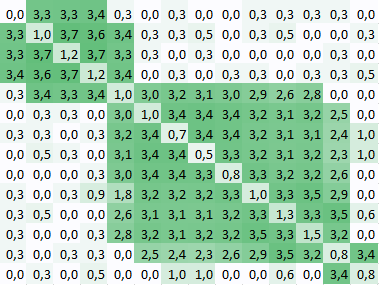
\includegraphics[width=0.6\linewidth]{gfx/noise.png}
    \caption{Observed noise in production data (logarithmic scale)}
    \label{fig:examplenoise}
\end{figure}

My method of dealing with the noise was to apply a threshold value to all the frequencies.
The value was a fraction $0 \le t_n < 1$ of the number of traces $N$ analyzed in the event log.
Any value in the matrix lower than $t_n N$ will be set to zero before the matrix is turned into a graph.
Similar thresholding will be performed when checking for parallelism (see definition \ref{def:logrelations}). 
For parallelism I calculate a fraction $d_p = \frac{f_\text{follow}}{f_\text{follow} + f_\text{precede}}$, where $f_\text{follow}$ is the frequency of follow relations from the upper triangle of the footprint matrix and $f_\text{precede}$ is the respective frequency from the lower triangle.
To counter noise, the relation is only considered to be parallel if the fraction is between the treshold values $t_p \le d_p \le (1 - t_p)$. 

Initial tests on the production data showed that relatively small ($t_n \le 0.01$) values were sufficient to counter the noise without affecting the model negatively. 
I used $t_n = 0.01$ and $t_p = 0.005$ to remove 1~\% of noise.

\nyi{Add figure for observed relations from excel}

\subsubsection{Latency}
\label{sec:latency}

In addition to discovering the process model, one of the requirements was to see statistics of the times each of the activities take. 
Since the event timestamps describe the end time for each activity, the length (or duration) of an activity can be found by comparing the timestamps of two consequent events. 
I call this time difference between events the \emph{latency}.
The latency describes how much time is expected to pass until an event is followed by another event.
The latency can be seen as the length of an edge in the directed graph.

The statistics the users were interested in were the ''top percentiles'' (TP).
A $n$-top percentile means the value that is higher or equal than $n\%$ of all the values in the set.
This can be expressed as the ''TPn'' value.
For example, the TP75 is the value that is higher or equal than 75~\% of all the values in the set.
TP50 corresponds to 50~\% and is equal to the median value of the set.
The top percentiles have proven to be more useful than for example averages, since the latencies 
in the store systems often had a very small amount of outliers with very high latencies, that skew the 
averages up.
The interesting statistics that were chosen are the TP50, TP75, and TP90. 
These correspond to the values used in other telemetry systems so they can be compared against each other for verification.

Programmatically the TP values can be found by ordering the values in the set in an ascending order as an array, and then picking the index that corresponds to the percentile. For example, is the ordered array has the length of 1000 elements, the TP90 value can be found at the 900th index.

When generating the graphs my method was to collect the statistics at the same time.
Since each cell in the footprint corresponds to an edge in the graph, I construct an array of latencies for each cell as I traverse through the traces.
When a number in the follow-frequency matrix is incremented, I also store the latency between the two events in the corresponding array. 
After the graph is generated, I can store the chosen key statistics (TP50, TP75, TP90) for each graph edge and discard the matrix and the arrays.

% directed graph tldr
The result of this method is a directed graph with nodes and edges.
Each node corresponds to an activity in the process model.
Each edge corresponds to a possible transition (pair of two consecutive events) in the trace.
The model can be verified by ''re-playing'' a trace. \nyi{elaborate?}
Each event in the trace should correspond to a valid directed edge, with the first event of the trace being at the input node of the graph.
The graph describes the process model that was discovered from the event log.

\nyi{figure for trace replay}

% implementation, paging
In my implementation I wanted to create a paged view that visualizes event based on the user's query.
For this reason I ran two nested database queries.
First, I run the user's query and retrieve the events, filtered by the user's permission level.
I sort these events by descending timestamp and pick five latest submission IDs.
These IDs will correspond to the five latest submission traces matching the user's query.
''Latest'' in this context means the traces with the most recent activity.
This query may also be paged, allowing the user to choose the next five traces, or any later set of five.
After five submission IDs has been retrieved, they are used to query all events belonging to these submissions. This results in five traces that can now be processed.

\subsubsection{Alternative methods}
\nyi{Maybe: Talk about implementing the alternative graph? not much to say..}\\
\nyi{Implementing the option of reading the graph shape from a JSON definition file}

\subsubsection{Storing the graphs}

As described before, the project allows the users to generate new graphs from any query supplied by the user.
Reading hundreds of thousands of events from the database, sorting them and generating the graph takes a lot of time, in the order of several minutes.
Since generating new graphs is resource-intensive, this functionality is restricted to the system administrators in Jury. 
Since Jury is an online tool the service response times need to be fast, preferably in the hundreds of milliseconds to preserve a smooth user experience \nyi{cite?}.
Generating the graph from a set of events for each web request from any user would be inefficient and the page load times would be in the order of minutes.
Because of this, I implemented two levels of caching in the system.

The Jury web server is distributed onto multiple server instances to provide high availability. The database server is shared between the instances.
Each generated graph is cached both in memory and in the database.
The in-memory cache is local to each instance and the database cache is shared.

Each cached graph is associated with a timestamp corresponding to the time when it was generated. 
This timestamp is used by the servers to determine when the cache is too old and should be refreshed.
For the in-memory cache this maximum age was chosen to be 15 minutes.
For the database cache the maximum age was set to 12 hours.
The long time was chosen since while the process model of the store system changes when improvements are made it will be in the order of days so a day old cached model will be accurate in most cases.

The cache system works as follows (in the perspective of a server instance):
\begin{enumerate}
    \item The server receives a HTTP request requiring a specific graph.
    \item The server reads the in-memory cache. \\
    \textbf{Less than 15 minutes old}: Return graph from memory to the user and stop. \\
    \textbf{Older than 15 minutes}: Return graph from memory to the user and continue to the next step in the background.
    \textbf{Graph not in memory}: Continue to the next step.
    \item The server reads the timestamp (age) from the graph stored in database\\
    \textbf{Less than 12 hours old}: Load graph from the database, store it in memory. Return to user if needed.
    \textbf{Older than 12 hours or not in database}: Move the graph timestamp in the database 15 minutes forward and generate a new graph. Once the task is finished, save it in the database, and in memory.
\end{enumerate}

This means that if the requested graph is in memory, it will be returned to the user immediately. If the version in memory is too old, a background task to retrieve or generate a new graph is started. This means that the user almost never has to wait for the page to load while the graph is being generated.
The only case when the user has to wait for the graph generation is if the instance has no graph in memory and the version in the database is also too old.
In practice this will only happen after a server restart when all the in-memory caches are purged.

The graph timestamp is moved 15 minutes forward at the start of graph generation to prevent a situation where two different server instances are generating the same graph separately.

This two-level caching improved the page loads from minutes to fractions of a second. Furthermore, since the graphs are now stored also in the same database as the events, they can be used in SQL queries. This proved useful, since SQL queries can be constructed to improve the notification functionality. See section \ref{sec:notifications} for more details about notifications.

\subsection{Real-time functionality}

Until this point I have considered the case of the event log, that corresponds to a time slice of past data.
This type of data can be seen as an ''aggregate'', since it will result in a model that describes events over a long period of time.
However, a key part of the analytics for the store is the ability to analyze and debug the current state of the system.
Without such functionality it will be difficult to analyze the state of the current submissions in the system.

As outlined before, the system already had a view to list events based on the user's query, as seen in figure \ref{fig:plaineventlog}.
I call this the \textbf{log view}.
The users of the system reported that this view was useful for debugging a specific issue for e.g. with a specific activity, but it does not provide a good overall view.
The request from the users was a view that shows a big picture of the status of a submission with the option to also drill down to the details.

% new small dataset from a query, often a single trace
My solution was to leverage the previously discovered aggregate model for visualization.
The model would be combined with the list of events returned by the query.
The aggregate model would be used to visualize the process, and the real-time data from the query would be ''overlayed'' on top of the model.

The method was to ''color'' the model with the data from the query.
The query results in a set of events that corresponds to the user's criteria.
For simplicity we can assume that the result is a single trace for an ongoing submission,
meaning that it is a set of sequential events that all belong to a single case.
In the full implementation the result can also be events from many separate submissions,
but the system handles it by splitting them into separate visualizations and then handling each one of them as a single trace.

In the beginning we create an ''colorless'' graph by copying the process model discovered earlier.
The colorless graph has a node for each activity and the corresponding graph edges between them.
The nodes are tied to the specific activities by including the Source and Subsource fields but they have no status, timestamp, or other metadata.
The visualization is ''colored'' by traversing through the trace in sorted order (ascending timestamp).
For each event in the trace, we find the corresponding node in the graph.
The node can then be ''colored'' by copying the status, timestamp, and other metadata from the event.
This can be repeated until we reach the end of the trace.
The result is a ''colored'' graph where all the activities that have been finished have a status and a time.
The nodes for the activities yet to come remain uncolored.

\nyi{graph coloring figure}

This graph can now be shown to the user.
The nodes are drawn on the screen as circles or rectangles, and the directed edges as arrows between them.
This is what I call the \textbf{graph view}.
The parallel nods are connected by double-sided arrows or an edge that otherwise indicates the parallelism.
In my visualization I took the ''colorization'' quite literally by having each status correspond to a color in the visuals. 
Uncolored nodes remained grey, completed nodes green or blue, nodes in progress yellow, and failed nodes red.
The colors help the user to get an immediate understanding of what the state of a submission is.
An example can be seen in figure \ref{fig:coloredgraph}.

\begin{figure}[htb]
    \centering 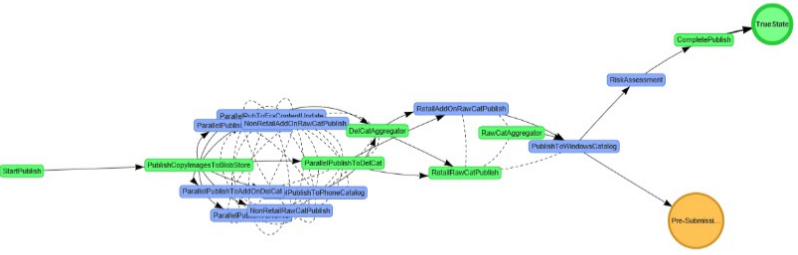
\includegraphics[width=0.9\linewidth]{gfx/graphcolor.png}
    \caption{Colored graph view}
    \label{fig:coloredgraph}
\end{figure}

\nyi{implementation details for overlays}

\subsection{Estimating the future}

One of the requirements discovered \nyi{where?} was to be able to provide estimations for the submission workflow completion times (labelled \emph{estimated time of arrival} or ETA). 
To provide such estimates I developed a method to traverse the graph forward after it has been colored.

% Estimating future on incomplete logs
The algorithm used in the project was a recursive traversal by using a stack.
The input for the algorithm is a graph which has been partly colored by a trace.
This means that some of the graph nodes have timestamps and metadata, while others (towards the end of the workflow) do not.
The goal is to use the previously generated process model to estimate
and fill in the data for the uncolored nodes.

% Statistical approach by using TP75
To fill in the data for future nodes, the algorithm needs a measure to be used for the estimation. 
This measure corresponds to the estimated ''edge length'' for each edge in the graph.
A simple approach is to use the statistical values that were collected during the graph generation process (see section \ref{sec:latency}).
The statistics are useful, since when giving time estimates we should aim for overestimating or giving the ''worst case'' guess \nyi{why?}.
For example, using the TP90 value should lead to an estimation that estimates the latencies in a way that overestimates 90~\% of the submissions.
However, choosing the right statistic should be considered since it is a trade-off between accuracy and overestimation \nyi{rephrase, citation needed}.
The plan was to use machine learning to improve the estimations (see section \ref{sec:ml-estimation}).

\nyi{pseudocode?}

% algorithm description
In theory, since all the graphs are workflow graphs, there should not be any loops \nyi{citation?}. 
In practice noise, errors, and changes in the system can lead to loops.
An empty list is initialized to keep track which nodes of the graph have already been visited.
The purpose of the list is to prevent a loop in the graph resulting in infinite execution.
First the algorithm finds the node which has the earliest timestamp.
This is treated as the graph start.
An empty stack is initialized and the start node is pushed into the stack.
After this initialization a recursive step is executed in a loop until the stack is empty.

The recursive step starts by popping a node (called the \emph{current node}) from the stack and checking if the node is valid.
This means checking that the node has not been visited already, that the node is not an error state, and that the node has a timestamp.
If the node has been visited already, it is ignored.
Error states are seen as anomalous, and since they often lead to the workflow being aborted, they should not be used for estimations.
The node needs to have a timestamp, otherwise there is no starting point for the estimation.
After the node has been deemed valid, it is marked as visited.

After the initial check all children for the node are retrieved.
This means finding all the edges that have the current node as the source, and collecting the nodes that the edges point towards.
For each of these nodes, the estimation is performed.
If the child node already has a timestamp from the coloration phase, it is ignored.
Otherwise, if the node is uncolored, the previously chosen edge length measure is used for the estimation. 
The length of an edge is a timespan, corresponding to an estimate for how much time will pass between the two events.
By adding the timespan to the timestamp of the current node, we get the estimation for the timestamp of the child node.

For parallel nodes (the nodes with a directed edge both to and from the current node) the step differs slightly. 
Since the activity corresponding to the node is known to be parallel to the current one, the edge length is seen as zero.
For this reason, the estimation step does not add anything to the timestamp but instead just copies the current node's timestamp to the parallel node.

After the timestamps of the child nodes have been estimated the child nodes are added to the stack and the step is performed again.
This continues until the stack is empty.
The stack will be empty when all the nodes connected to the starting node have been visited.
This means that barring error states every node will now either be colored or have a timestamp estimation.
These estimations can be shown to the user when the graph is visualized.

\nyi{implementation details for estimation}\\
\nyi{What is different when using a predetermined JSON shape}

\subsubsection{Timeline view}

\begin{figure}[htb]
    \centering 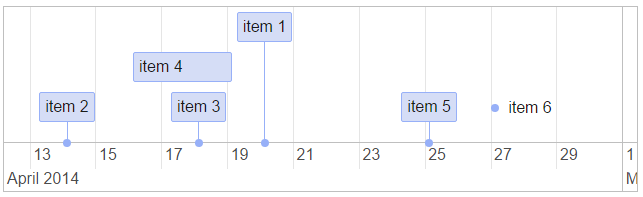
\includegraphics[width=0.6\linewidth]{gfx/basictimeline.png}
    \caption{A basic example of a ''timeline'' \nyi{make a better one}}
    \label{fig:basictimeline}
\end{figure}

During the protyping phase I discovered that the directed graphs were not intuitive to read for the users.
Trying to manipulate the graph shape and selecting each node to see the details turned out to be cumbersome.
Two users wished for a ''sorted'' view in the initial tests.
The sorted view should show the events arranged horizontally across the screen by time.
This resulted in the second prototype which I labelled the \textbf{timeline view}.
A basic example of what a timeline is can be seen in figure \ref{fig:basictimeline}.
The timeline has items set on a horizontal axis.
The horizontal axis corresponds to time, with past being on the left and the future on the right.
The vertical axis has no meaning other than to separate the parallel items visually to help the user see which activities happen in parallel.

% Generating a timeline view with start and end times from the overlay
As can be seen from the figure, each item in the timeline has a width.
This means that the items have a both a \textit{starting time} and an \textit{ending time}.
However, in the event log each event only has a single timestamp.
The event timestamp corresponds to the ending time of an activity.
For the purposes of the timeline, it does not matter whether the timestamp comes from the log or whether it is an estimation.
To find the starting times, we can leverage the process model graph again.

% Methods of finding the start times and dealing with parallelism
In my project I made the assumption that switching tasks takes a negligible time.
This means that when a task ends, the next task begins immediately.
With this assumption we can discover the starting time by looking at the end time of a previous task.
We can find the previous task by following the graph edges backwards and finding its dependencies.
Choosing the latest ending time of these dependencies results in the starting time of the activity.
In this method, all parallel tasks are treated equal, so each activity also must take into account all dependencies of its parallel tasks.
In the case where there are no dependencies (such as the first activity of the graph) a predetermined length will be used as a fallback.

In other words, before this step the timeline has all events as zero-width with only the end times. The algorithm sets the start time to be the earliest possible time without breaking the restrictions given by the process model dependencies.
After this step, all items in the timeline correspond to an activity in the workflow. Furthermore, all items have a start time and an end time.
When the timeline is visualized, the items where the timestamp is an estimation can be separated by color or other means.
Furthermore, since the horizontal axis corresponds to time, the current time of the user can be shown as a vertical line.
This helps to highlight the current time to the user and to separate future estimations from observed events.

\nyi{add picture of a finished timeline}

\nyi{timeline implementation details}

\subsection{Machine learning}
\label{sec:ml-estimation}

% How ML approach could be used to improve the statistical approach
After I had implemented the statistical estimation, the next step was to research whether it could be improved by using machine learning. 
The idea was that for each graph edge, instead of using a statistical value to estimate the length, a machine learning model could be used.
The model could take into account the current time and transition, in addition to other characteristics of the submission such as details about the application package.
The hypothesis was that characteristics such as the application package size have a predictable effect on the latencies.

To test this hypothesis I collected a set of training data from the production environment and used it to train and test machine learning models.
Had the model accuracy been proven to be more accurate than the statistics, the model could have been deployed to the production system.

% Explain training dataset generation
The training dataset was generated from a time slice of the event logs. 
By using both a predetermined (JSON) process model \nyi{should be introduced somewhere before} and the automatically discovered process model, two datasets were created. The dataset contained the observed values for the latencies, labelled by the activity transition and the application it belongs to.
These rows were then joined with a dataset of known applications and their characteristics to create the final training data.
The resulting dataset consisted of 16 columns of features such as the package size and the current transition (activity being observed), and a label column corresponding to the measured latency in seconds. \nyi{does this need a concrete listing?}
The data was filtered to only contain measurements from valid traces with the requirement of having no errors and conforming to the process model.
The datasets used contained \nyi{XX~XXX} rows for the JSON template, and \nyi{XX~XXX} rows for the automatically discovered template.

% Explain models used (poisson \cite{azurepoisson}, bdt \cite{azurebdt} \cite{lambdamart2010})
% data suitability
% result interpretation
The machine learning models used in training were Poisson Regression \cite{azurepoisson} and Boosted Decision Trees \cite{azurebdt}.
\nyi{add: compared/contest, not together}
These were chosen based on a few factors.
The first factor was that the model needs to suit the data.
Since the latencies are values of time measured as activity durations, they fall on a Poisson distribution. 
This is why a Poisson Regression model was selected.
The Boosted Decision Trees model had been used before in the store for application classification with good results, so it was believed to work well with application characteristics.

Second factor for choosing the models was the interpretability of the results.
Since this project was experimental and there was no baseline, I wanted to be able to inspect the models and reason about their characteristics.
Since both the Poisson Regression model and the Boosted Decision Trees output the per-feature weights for the model, they can be inspected and reasoned about.
Compared to something like a neural network, which is highly challenging for humans to interpret \nyi{citation needed} this is a clear advantage.
The best model based on prediction accuracy was to be chosen for an in-production test.

% accuracy
% training / regression speed
The average error and the mean square error values were to be used to evaluate model accuracy \nyi{maybe elaborate}.
Lastly, if multiple accurate models was to be found, the model training and regression performance would be used to evaluate them.

\begin{figure}[htb]
    \centering 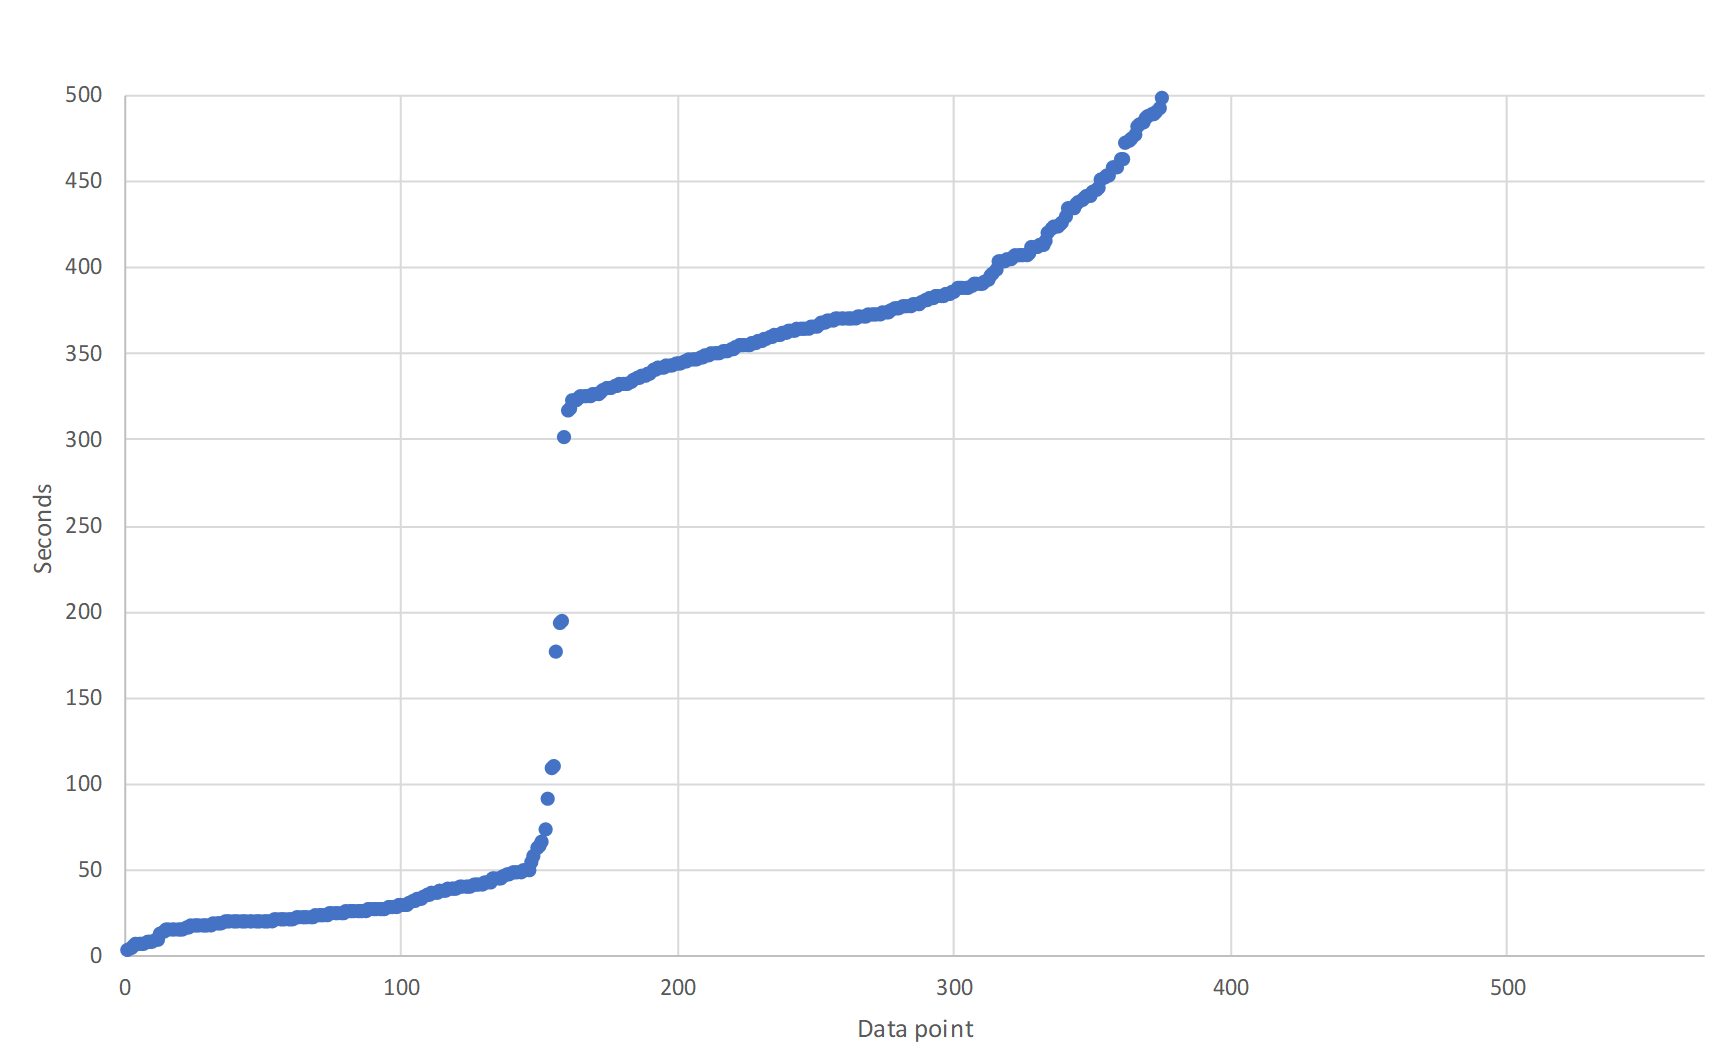
\includegraphics[width=0.6\linewidth]{gfx/resubmissions.png}
    \caption{Latency distribution for resubmissions \nyi{remake}}
    \label{fig:resubmissions}
\end{figure}

% Explain initial testing
% Testing with noisy features removed (textual fields)
The features used in the data were chosen based on experimental testing and domain knowledge.
Initially, 12 features read from the application package characteristics where used. The features were numeric and boolean describing the package size, the capabilities required, and other features that would be available immediately at the start of the submission.
Furthermore, two features read from the event logs were added.
These were an enumerator for the current transition (activity being measured) and the time passed since the beginning of the trace.
The label column was the measured latency.
Initially, data also included other fields such as the application description, keywords, and other developer-supplied (mostly textual) information. 
However, these were deemed noisy and resulted in overfitting.
They also drastically increased the training time because of n-gram generation.
The domain experts (the system engineers) knew to inform that those fields are not used in the ingestion pipeline so they were removed resulting in the 12 features.

% Explain additional features
% identical resubmission
After the initial testing, two additional features were added to the dataset.
The first additional feature was a boolean value describing whether the application package is identical to the previous submission.
This was because the domain experts knew that this would lead to some of the activities skipping execution internally, drastically reducing the execution time for a couple specific activities. 
This was also clearly seen in the data when the latency distribution for an activity were plotted. 
This can be seen in figure \ref{fig:resubmissions}. 
With this graph the training data could be split into two sets labelled by whether the submission is an identical resubmission.
%  posting that needed human interventiondcxfkkkkkkkkkkkkkkkkkkm
%                                       a cat did this ^ 
The second additional feature was whether the application ingestion triggered a manual review (human curation). 
Since orchestrating human manual reviewers contains overhead, a manual review is known to delay the ingestion time considerably.
This can also seen from a latency distribution graph as a clear difference for some other steps (see figure \ref{fig:manualreview}).
This was used similarly to add the manual review boolean feature into the dataset.
I performed more tests with these additional features to test whether they improved model accuracy.

\begin{figure}[htb]
    \centering 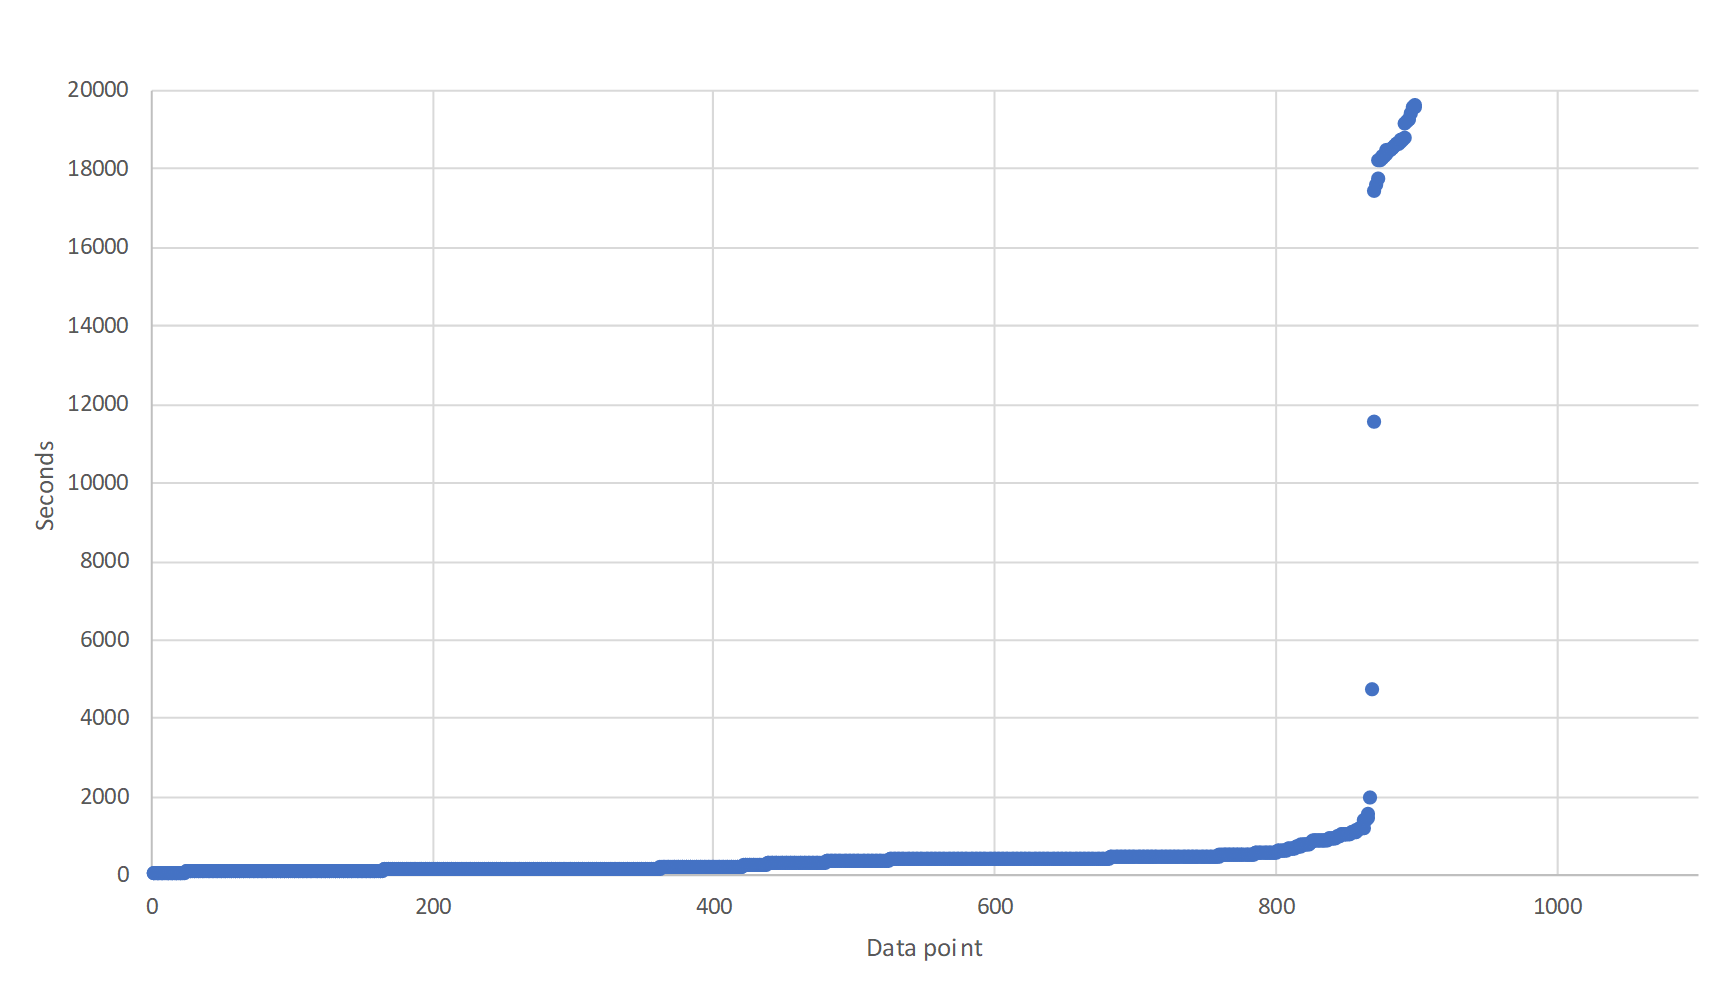
\includegraphics[width=0.6\linewidth]{gfx/manualreview.png}
    \caption{Latency distribution for manualreview \nyi{remake}}
    \label{fig:manualreview}
\end{figure}

\subsection{Notifications}
\label{sec:notifications}

\nyi{Describe how the estimates could be used for notifications}

\subsection{User interface}

\nyi{description of user interface}\\
\nyi{user interface features discovered at mid point}

\nyi{vis js, asp.net mvc, etc}\\
\nyi{ - displaying the graph}\\
\nyi{ - merging of ''bubbles''}\\
\nyi{ - timeline view}\\
\nyi{ - multiple graphs/timelines per page}\\

\nyi{Make sure the difficulties are all mentioned somewhere}\\
\nyi{(you'll want these for the presentation)}\\
\nyi{ - parallelism}\\
\nyi{ - clock skew}\\
\nyi{ - changes in workflow}\\
\nyi{ - bugs manifesting in graphs (is this really a bad thing?)}\\
\nyi{ - dealing with rare events (manual review)}\\
\nyi{ - confidentiality}